\chapter{绪论}\label{chap:introduction}
\setcounter{algorithm}{0} % 重置算法计数器
\hypersetup{
    citecolor=black, % 设置引用日期为黑色
    linkcolor=black,   % 设置普通链接颜色
    urlcolor=black % 设置网址链接颜色
}


\section{课题研究背景}
随着我国新型城镇化战略和区域协调发展战略的深入推进，城市群与都市圈已成为国家高质量发展的核心载体。作为支撑高频次、大容量、快速化城际出行的骨干交通方式，城际高速铁路近年来实现了跨越式发展。以京津冀、长三角、粤港澳大湾区等典型区域为代表，城际线路普遍采用高密度、公交化、周期化运营模式，列车追踪间隔压缩至3–5分钟，日均开行对数可达百对以上，形成了高度耦合、强动态交互的复杂运行系统。在此背景下，保障列车运行的准点性、稳定性与鲁棒性，不仅关乎运输效率与乘客体验，更直接关系到整个区域综合交通网络的韧性与可靠性。然而，这一目标的实现正面临来自外部环境日益严峻的扰动挑战，其中由客流波动引发的停站时间不确定性，已成为影响城际高铁运行秩序最突出、最难以规避的核心因素\cite{wang2021,zhang2021train,zhang2023multistage}。

与城市轨道交通不同，城际高铁具有站间距长、单程运行时间久、客流潮汐特征显著等特点。在实际运营中，上下车客流规模受通勤规律、节假日出行、大型活动乃至突发公共事件等多重因素影响，呈现出高度的随机性、结构性与突变性\cite{yu2023distributed}。例如，在早晚高峰时段，特定车站可能短时间内涌入大量旅客，导致实际停站时间远超计划值；而在平峰期，客流稀疏又可能使列车提前完成乘降作业。这种由客流扰动引起的停站时间偏差，虽看似微小，却会在高密度追踪运行环境下通过“前车延误—后车等待—间隔压缩”的连锁机制迅速传播并放大，形成所谓的“蝴蝶效应”，最终导致大面积、长时间的运行图失序。尤其在环形或端点折返式运营结构中，延误甚至会跨周期累积，严重破坏周期化运行的内在稳定性\cite{tiong2023analyzing,yun2009decision}。

面对此类扰动，传统调度方法主要依赖离线优化模型，如混合整数线性规划（MILP）、启发式算法或仿真优化等，试图在延误发生后重新生成全局最优运行图。尽管这类方法在理想假设下能获得较优解，但其计算复杂度随列车与车站数量呈指数级增长，难以满足高密度场景下秒级响应的实时性要求。更重要的是，它们通常将客流视为确定性参数或简单随机变量，未能充分刻画其半稳态周期性（如每日重复的早晚高峰模式）或突发性（如临时集散事件）的内在动态特性，导致调度方案在真实复杂环境中适应性不足。近年来，基于控制理论的实时反馈调度方法因其低计算负担与在线适用性受到广泛关注\cite{DIAS201698,Stankovic2001,Walsh2001,Stankovic1999,SHOBRYS2002149}。然而，现有研究多建立在地铁或干线铁路的简化模型之上，普遍假设“单区间单车”（即列车数小于车站数，M < N），而城际高铁在高峰时段常出现“多车同区间”（M > N）的运行状态，使得传统模型无法准确描述列车间的时空耦合关系，进而导致控制策略失效。

更为深层的挑战在于，现有实时控制方法在处理客流扰动时仍存在理论与实践上的显著鸿沟。一方面，鲁棒控制策略（如H∞控制、滑模控制）\cite{hansen2001robust,calafiore2012robust,weinmann2012uncertain,mhaskar2006robust,mayne2005robust,grimm2007nominally,dorato2003historical}虽能在最坏扰动情形下保证系统稳定，但其设计往往过于保守，牺牲了正常工况下的调度性能，难以兼顾效率与安全；另一方面，尽管系统在日复一日的周期化运行中积累了大量历史数据，蕴含着丰富的客流统计规律与运行经验\cite{li2019short,daamen2004modelling,sun2015integrated,zhang2017real}，但当前方法普遍缺乏有效的学习机制，无法将这些先验知识转化为自适应调控能力，致使重复性偏差反复出现、无法根除。此外，当客流模式在不同工况间切换（如平峰→高峰→恶劣天气）时，单一控制律难以兼顾多场景下的最优性能，亟需引入能够识别运行状态并动态调整策略的智能机制。

正是在上述现实需求与理论瓶颈的双重驱动下，本研究聚焦于构建一套面向不确定与突变客流的城际高铁列车实时重调度控制体系。该体系以精确刻画M > N运行特征的状态空间建模为基础，融合鲁棒模型预测控制对有界扰动的抗干扰能力、迭代学习控制对周期性偏差的渐进消除能力，以及模糊逻辑对多工况切换的自适应表征能力，旨在实现从“被动抗扰”到“主动学习”再到“智能融合”的跨越。通过这一系统性探索，不仅有望突破现有方法在扰动抑制、实时响应与性能优化方面的局限，更将为高密度轨道交通系统的自主调控提供一套兼具理论深度与工程价值的新范式，助力我国智能高铁向更高水平的安全、高效与韧性迈进。           


\section{国内外研究现状}
%在当前故障诊断领域，异常检测与鉴别技术正逐步成为提升系统安全性和可靠性的关键研究方向之一。%国内外学者围绕基于模型、信号处理与数据驱动的方法展开了广泛探索，旨在实时捕捉并准确定位系统中的异常现象。本文研究的异常信号主要包括物理故障和网络攻击，其中物理故障指设备或系统在运行过程中因内部或外部因素而产生的异常状态，而网络攻击则涉及通过网络入侵或干扰对系统造成的安全威胁。

尽管城际高铁列车重调度主要面向客流扰动或运行干扰等不确定性场景，但其本质仍是在动态约束下实时生成满足安全与效率要求的列车运行调整方案。因此，首先对现有列车运行方案制定方法进行系统梳理，以阐明本文为何选择基于先进控制理论的框架（后续简称“基于控制的方法”）来求解该问题。随后将深入分析现有基于控制的方法在应对城际高铁高密度、M>N运行特性及复杂客流扰动时所面临的挑战，特别是模型适配性不足与扰动处理能力有限的问题，以此为构建面向客流特性的精细化建模与分层抗扰控制机制提供研究动机。最后进一步探讨现有研究如何刻画和保障调度方案的鲁棒性与自适应性，并剖析现有控制策略在兼顾稳定性、实时性与性能优化方面的局限，为本文开展融合鲁棒模型预测控制、迭代学习与模糊逻辑的协同优化研究奠定理论基础。


\subsection{高速列车运行调整方法总体研究现状}

\textbf{(1) 数学规划方法}

数学规划方法是列车调度领域研究最早也是发展最为成熟的一类方法。Szpigel 首次提出单线铁路列车调度的整数规划模型，为后续研究奠定基础\cite{Szpigel1973}。此后，大量学者相继加入该领域，提出了多种建模方法与求解算法。在模型构建方面，现已形成包括混合整数线性规划模型（Mixed Integer Linear Programming, MILP）\cite{earl2005iterative,birgin2014milp,yao2023novel,meng2023milp}、约束规划（Constrained Programming）\cite{chen2024data,wang2022adaptive,rossi2008constraint,li2008chance}以及替代图模型（Alternative Graph Model, AG）\cite{ruiz2017alternative,zhang2022graph,robins2010alternative}等在内的多样化建模范式。随着路网复杂度不断提升，相关研究也持续深化：D’Ariano 等人 \cite{DAriano2007} 构建了面向实际铁路网络的微扰恢复 MILP 模型，并结合分支定界算法实现高效求解；Zhao 等人\cite{Zhao2020}提出了一种基于区段的协同优化方法，以节省高速列车的运行时间和能耗；Zhang 等人\cite{Zhang2023}针对中断期间采用座位预留机制的铁路系统，建立了一个包含补偿机制的整数线性规划模型，以提供更优的整体解决方案。此外，Ghasempour 等人\cite{Ghasempour2020}展示了基于近似动态规划（ADP）构建的自适应交通控制器在局部部署后对全路网产生的影响，该控制器用于实时运行管理；Liu 等人\cite{Liu2024}则针对复杂多线网络中受风速限制条件下的列车运行图调整（TTR）问题，提出了一种成本低廉且精度足够的代理模型；Yin 等人\cite{Yin2023}构建了一种灵活的定向列车调度框架，整合时刻表重调度、侧线及粮仓专用车辆段策略。在控制与优化层面，Huang 等人\cite{Huang2021}针对高速列车速度与位移跟踪中的未知时变参数和集总不确定性，设计了基于自适应迭代学习的控制方案；Liu 等人\cite{Liu2019}则提出一种时刻表优化方法，协调地铁系统中列车的加速与制动过程，以在不依赖储能装置的前提下最大化再生能量利用。为提升计算效率，Pellegrini 等人 \cite{Pellegrini2014} 和 Lamorgese 与 Mannino \cite{Lamorgese2015} 分别发展了基于 Benders 分解与列生成的精确算法，显著缩短求解时间；Leutwiler 等人 \cite{Leutwiler2023} 进一步利用延误相似性加速逻辑 Benders 分解，在扰动响应速度上取得突破。近年来，学者们在经典模型基础上不断拓展，开发出能够应对更加复杂调度场景的新型数学模型，推动了列车调度理论与实践的深度融合。


\textbf{(2) 仿真器模拟方法}

目前基于仿真器模拟的方法在高铁调度中也有所探索。Shakibayifar 等人\cite{Shakibayifar2017}提出了一种结合动态调度优先规则的仿真优化模型。Zhou 等人\cite{Zhou2021}提出了一种多阶段智能方法，利用改进的迁移学习和集成学习增强的随机向量函数链接网络（RVFLNs）来预测列车延误的动态变化及其传播规律；在获得延误预测结果后，进一步构建更完善的仿真模型用于重调度。Petersen 等人\cite{Petersen2010}建议采用计算机仿真技术对列车调度问题进行建模。Hou 等人\cite{Hou2019}通过引入二元变量作为地铁信号供应商的选择指标，在车载自动列车运行（ATO）系统中预设 ATO 运行曲线，建立了用于地铁时刻表重调度的混合整数规划（MIP）模型。在此基础上，大量学者将仿真作为核心评估或驱动引擎，嵌入各类调度求解流程。Hassannayebi 等人\cite{hassannayebi2021simulation} 明确构建了一个面向快速轨道交通的仿真-优化集成框架，其中微观仿真器用于动态评估重调度方案的运行效果，并反馈指导优化迭代。Luethi 等人\cite{luethi2009structure} 设计了一套基于仿真的实时重调度系统，通过仿真环境对多种调度规则进行在线测试与性能比较，从而支持动态决策。Altazin 等人\cite{altazin2020multi} 在求解高密度铁路多目标重调度问题时，依赖仿真平台验证解的可行性与鲁棒性，并将仿真结果作为优化目标的重要组成部分。Tamannaei 等人\cite{tamannaei2016novel} 虽采用模拟退火算法求解双线铁路重调度模型，但其方案有效性完全通过定制化列车运行仿真器进行验证，强调仿真在策略评估中的不可替代性。Eaton 等人\cite{eaton2017ant} 将蚁群优化应用于铁路枢纽动态调度，其算法在动态仿真情境下运行，实时响应由仿真生成的列车位置与冲突信息，实现闭环调度。更早地，Cheng\cite{cheng1998hybrid} 提出的混合仿真方法，直接将仿真作为解决资源冲突的核心机制，通过模拟列车占用轨道区段的过程，动态触发调度调整。

\textbf{(3) 智能学习方法}

%智能算法也有多种方法被应用于高速铁路重调度。Yue 等人\cite{Yue2023}提出了一种基于强化学习的高速列车实时重调度方法；Krasemann等\cite{Krasemann2012}采用贪心算法求解重调度方案；Ning 等人\cite{Ning2019}则引入深度强化学习方法，以最小化铁路线上所有列车的平均总延误。Wenliang 等人\cite{Wenliang2015}提出了一种启发式智能算法，在多周期混合运行条件下优化列车运行时间。Khadilkar\cite{Khadilkar2019}采用启发式算法研究了多周期混合工况下高速列车的运行时间优化问题。Li 等人\cite{Li2014}提出了一种基于恢复时间、原始时刻表及轨道替换成本估算的替代轨道调度方法，以解决轨道中断后容量恢复时间随机的问题。Oneto 等人\cite{Oneto2017}利用浅层与深层极限学习机进行列车延误预测。Isaai 等人\cite{Isaai2000}提出了一种基于约束的启发式算法用于旅客列车延误预测。Xu 等人\cite{Xu2023}提出了一种两阶段宏观调控方法，包含策略引导的决策阶段和基于 Transformer 的建模阶段。Dong 等人\cite{Dong2025}提出了一种深度强化学习方法，旨在减少整条铁路线上列车的总延误。

近年来，智能学习方法因其在处理高速铁路列车运行调整中多目标、非线性和强耦合特性方面的良好适应性，逐渐成为重调度研究的重要技术路径。该类方法的发展可划分为两个阶段：早期以元启发式优化算法为主导，近期则转向以数据驱动的学习机制为核心。
元启发式算法因具备较强的全局搜索能力且对问题结构先验依赖较低，在复杂调度场景中展现出独特优势 \cite{Cuevas2023}。已有研究广泛采用禁忌搜索\cite{Corman2010}、遗传算法（GA）\cite{WangR2023}、粒子群优化（PSO）\cite{WangR2023,Hassannayebi2018} 以及蚁群优化（ACO）\cite{ZhouXZ2018,Behiri2023} 等方法求解列车重调度问题。为进一步提升性能，学者们提出了多种混合策略：例如，Wang M 等人融合 GA 的全局探索与 PSO 的局部精细搜索能力，构建了收敛效率更高的混合优化器\cite{WangM2019}；Schachtebeck 等人则利用元启发式生成高质量初始解，为商业求解器（如 CPLEX）提供热启动支持，从而加速数学规划模型的求解过程\cite{Schachtebeck2008}；另有工作结合项目评估与审查技术（PERT）界定可行调度窗口，并借助模拟退火在缩减空间内高效寻优\cite{Norio2005}。此外，Krasemann\cite{Krasemann2012} 设计了基于贪心规则的快速响应机制；Wenliang\cite{Wenliang2015} 与 Khadilkar\cite{Khadilkar2019} 针对多周期混合运行模式分别提出了运行时间优化的启发式方案；Li\cite{Li2014} 则针对轨道中断后容量恢复不确定性，构建了替代路径调度策略；而 Isaai\cite{Isaai2000} 和 Oneto\cite{Oneto2017} 分别利用约束启发式与极限学习机开展列车延误预测，为调度决策提供支撑。
然而，上述方法仍高度依赖人工设计的搜索逻辑或经验规则，难以从历史运行数据中自主提炼调度知识。随着人工智能技术的进步，基于学习的智能决策方法为突破这一局限提供了新思路。强化学习（Reinforcement Learning, RL）自 20 世纪 80 年代由 Sutton 等人系统提出以来，受限于计算资源长期未能广泛应用。直至深度学习兴起，RL 在复杂序贯决策任务中的潜力才被充分释放——以 AlphaGo 在围棋领域的突破为代表，其成功验证了 RL 处理高维状态-动作空间的能力，并推动其向交通优化等现实场景迁移\cite{Haydari2020,WangQ2021,Cao2020}。目前，RL 在列车调度中的应用主要体现为两类范式：一是增强传统优化求解器，如用于指导分支定界中的变量选择\cite{Qu2022} 或优化割平面生成策略\cite{Tang2020}；二是直接输出调度指令，即训练智能体端到端地完成运行调整。后者更契合实时性要求：Šemrov 等人\cite{semrov2016reinforcement} 首次将 Q-learning 应用于单线铁路重调度，使代理能模拟调度员行为；Yue\cite{Yue2023} 与 Ning\cite{Ning2019} 分别构建了基于 RL 与深度 RL 的高速列车重调度框架，以最小化系统总延误；Dong\cite{Dong2025} 进一步提出深度强化学习架构，实现全线列车协同优化。Xu\cite{Xu2023} 则结合策略引导与 Transformer 模型，设计了两阶段宏观调控机制。Liao 等人\cite{Liao2021} 还针对扰动下的节能重调度问题，开发了深度强化学习方法。



\subsection{基于周期性时刻表调度研究}
周期性运行模型具有明显的规律性，包括停站模式、列车运行计划及运行方式。目前已有部分关于周期性列车运行的研究成果。Sartor 等人\cite{Sartor2023}提出了一种用于准周期性战略列车时刻表编制的混合整数线性规划（MILP）模型，为在多种场景下优化列车时刻表提供了思路。Cacchiani 等人\cite{Cacchiani2012}探讨了利用周期性事件调度问题等方法优化周期性时刻表，以最小化乘客等待时间，并基于周期性基础构建了整数线性规划模型。Zimmermann 等人\cite{Zimmermann2003}考虑了固定间隔重复服务的公共交通铁路周期性时刻表，提出了一种应对冲突需求并降低成本的方法。Caimi 等人\cite{Caimi2011}提出了一种两层方法，用于生成无冲突的周期性列车时刻表，并对 PESP 进行了扩展，允许使用灵活的时间窗口而非精确时刻。Gromann 等人\cite{Gromann2012}将周期性调度问题（如列车时刻表）编码为布尔可满足性（SAT）问题，并证明该方法优于传统的基于约束的方法，能够建模更大规模的实际场景。Ai 等人\cite{Ai2022}提出了一种基于深度强化学习的公交时刻表动态优化方法，但其重点在于时刻表设计，而非延误发生后的重调度。在地铁线路的周期性运行方面，也有可供参考的方法。

在地铁线路的周期性运行方面，也有可供参考的方法。Besinovic 等人\cite{Besinovic2022}提出了一种集成的中断管理模型，将列车重调度与客流控制相结合。针对给定的时变客流需求矩阵，Niu 等人\cite{Niu2015}建立了一个带线性约束的统一二次整数规划模型，通过将各车站的有效乘客上车时间窗与列车到发时刻同步，以最小化乘客在站总等待时间。Hu 等人\cite{Hu2023}旨在解决列车时刻表重调度、客流控制与地铁线路越站运行模式的协同优化问题，提出了一个混合整数非线性规划（MINLP）模型，在服务水平与运营成本之间实现性能平衡。Shao 等人\cite{Shao2022}在保障出行效率与成本合理性的前提下，提出了一个综合优化模型，联合优化列车时刻表与停站方案，以最小化乘客总旅行时间、列车运行时间，并提升系统公平性。Van Breusegem 等人\cite{VanBreusegem1991}提出了面向地铁线路的状态空间模型与反馈控制器。Wang 等人\cite{Wang2022}提出了一种两阶段模型，专注于市域列车的分布式实时重调度。Yang 等人\cite{Yang2016a}基于 Takagi-Sugeno (T-S) 模糊双线性控制模型（该模型综合考虑了系统的安全性、准点性和能效），研究了一种自适应预测控制方法。Li 等人\cite{Li2013}提出了一种基于梯度的外点法，用于构建最优驾驶策略。Yang 等人\cite{Yang2016}基于随机规划构建了一个地铁系统时刻表与速度曲线联合优化模型，通过考虑列车质量、牵引力和运行阻力等方面的不确定性，实现了显著的节能效果。上述周期性时刻表方法均采用优化方法求解，计算量大、求解耗时长。在列车密度高、运行密集的城际高速铁路（HSR）场景中，难以满足实时时刻表重调度的需求。特别是在高密度环形周期运行线路中，需决策的车站数量较多，导致优化决策变量急剧增加，计算时间显著延长。。

\subsection{目前现代控制理论应用}
近年来，以模型预测控制（MPC）、迭代学习控制（ILC）以及模糊控制为代表的现代控制理论在众多工程领域得到了广泛应用，为复杂动态系统的实时优化与鲁棒调控提供了重要理论基础和技术支撑。模型预测控制作为一种先进控制策略，通过构建显式系统模型对未来状态进行预测，并在有限预测时域内求解优化问题以获得最优控制输入。该方法能够有效处理多输入多约束系统，并具备一定的鲁棒性\cite{Garcia1989,Maciejonski1999}，因此在交通运输系统调度与优化问题中具有良好的应用前景。Rosolia 等人\cite{Rosolia2022a}提出鲁棒学习型模型预测控制方法，用于不确定系统中的重复性任务执行。在轨道交通实际运行环境中，乘客流量波动及各类运行干扰普遍存在，因此控制策略必须具备足够的鲁棒性以应对不确定性。基于此，鲁棒 MPC 被认为是实现列车调度优化的重要手段\cite{Kothare1996}。Liu 等人\cite{Liu2023}构建了以乘客为中心的城市轨道交通网络乘客同化模型；Li 等人\cite{Li2016}针对存在客流不确定性与运行干扰的地铁线路，设计了鲁棒 MPC 重调度方法，实现了列车运行的实时优化。随着研究的深入，MPC 与 ILC 的融合逐渐成为热点方向。针对重复运行场景，Zheng 等人\cite{Zheng2023}提出空间自适应终端迭代学习预测控制方法，用于执行器饱和条件下的列车自动停车问题；Zhang 等人\cite{Zhang2021}针对存在不确定性的批处理过程，提出二维模型预测迭代学习控制策略以提升系统控制性能；Wu 等人\cite{Wu2022}构建了数据驱动型迭代学习预测控制框架；Ma 等人\cite{Ma2021}利用控制仿射前馈神经网络提取历史批次数据特征，建立非线性模型，为当前批次控制器设计提供支持。在铁路系统研究领域，已有文献\cite{Yang2009,Wang2020}将乘客流量建模为模糊变量，从而将系统描述为模糊系统。相较于将客流需求视为确定值或随机变量的传统建模方式，模糊建模能够更合理地刻画实际运营中的不确定性与信息不完备性，因此具有较强的现实意义。
在此基础上，模糊控制与 ILC 及 MPC 的融合研究不断发展。Precup 等人\cite{Precup2008}将迭代学习算法与 Takagi–Sugeno 型 PI 模糊控制器相结合，强调了工程实现的可行性与系统效率。Wang 等人\cite{wang2004direct}提出基于输出递归模糊神经网络的直接自适应迭代学习控制方法，通过在线逼近系统不确定性提升了控制精度与收敛性能。Chien\cite{chien2008combined}针对控制任务变化问题设计组合自适应律的模糊 ILC 方法，提高了系统对任务变化的适应能力。Han 等人\cite{han2023iterative}进一步将模糊神经网络引入迭代学习模型预测控制框架，在提升预测精度的同时增强了系统鲁棒性与学习收敛性能。


\section{存在问题和本文主要工作}
综上所述，尽管现有研究在列车运行调整方法上取得了丰富成果，涵盖数学规划、仿真优化、智能学习及现代控制等多个技术路径，但在面向高密度城际高速铁路（M > N）这一典型场景时，仍存在以下关键问题亟待突破：

1)模型适配性不足：传统基于控制理论的重调度方法多建立在“单区间单车”（M < N）的简化假设之上，难以准确刻画城际高铁高峰时段“多车同区间”的复杂时空耦合关系，导致状态空间建模失真，进而影响控制策略的有效性与安全性。

2)扰动处理能力单一：现有方法对客流扰动的建模过于理想化——或视为确定性偏差，或简化为随机噪声，未能同时兼顾其半稳态周期性（如每日重复的早晚高峰）与突发突变性（如大型活动、极端天气）的双重动态特性，致使调度方案在真实复杂环境中适应性不足。

3)控制策略缺乏协同机制：鲁棒控制虽能保障最坏情形下的系统稳定，但往往过于保守，牺牲正常工况下的运行效率；迭代学习控制可有效消除周期性偏差，却对非重复性扰动无能为力；而模糊逻辑虽具备多工况自适应潜力，但缺乏与优化控制的深度融合。三者各自为政，尚未形成“抗扰—学习—适应”一体化的协同调控框架。

4)实时性与性能难以兼顾：数学规划与仿真优化方法虽能获得高质量解，但计算复杂度高，难以满足秒级响应的实时调度需求；而现有实时控制方法又常因模型简化或策略单一，导致性能次优，难以在稳定性、实时性与运行效率之间取得平衡。

针对上述挑战，本文立足于高密度城际高铁运行实际，以先进控制理论为核心，提出一套融合鲁棒性、学习性与自适应性的列车实时重调度控制体系。具体研究工作包括：

1)构建面向 M > N 运行特征的精确状态空间模型：突破传统“单区间单车”假设，建立能够准确描述多列车在共享区间内动态交互关系的离散时间状态空间模型，为后续控制器设计提供可靠基础。

2)提出鲁棒模型预测控制（RMPC）：针对有界但未知的突发性客流扰动，设计基于 Tube-MPC 思想的鲁棒控制器，确保系统在最坏扰动下仍满足安全间隔与准点约束，提升抗干扰能力。

3)引入迭代学习控制（ILC）：利用城际高铁日复一日的周期化运行特性，设计基于批次更新的 ILC 机制，对重复性停站延误进行渐进式消除，实现“越跑越准”的自主优化能力。

4)构建模糊逻辑驱动的多模态切换机制：通过模糊规则识别当前运行工况（如平峰、高峰、恶劣天气），动态调整 MPC 与 ILC 的权重与参数，实现控制策略在不同扰动模式下的自适应切换与性能最优。

5)开展多场景仿真实验验证：基于典型城际线路（如京津、沪宁等）构建高保真仿真平台，对比分析所提方法在扰动抑制效果、计算耗时、准点率提升及能耗表现等方面的综合性能，验证其工程可行性与优越性。

通过上述系统性研究，本文旨在实现从“被动抗扰”到“主动学习”再到“智能融合”的跨越，为高密度轨道交通系统提供一套兼具理论严谨性、算法实时性与工程实用性的新型重调度控制范式，助力我国智能高铁向更高水平的安全、高效与韧性迈进。

%此外，目前国内外对于多智能体系统中网络攻击与物理故障的检测和鉴别的相关研究还相对较少。现有的一些基于分布式观测器的异常检测和鉴别框架需要待检测节点向其邻居发送一些隐私信息。此外，这类框架需要待检测节点的邻居节点之间进行二次信息交互，且此类框架存在一个假设条件就是邻居节点之间的二次信息交互过程中不会受到网络攻击。这个假设显然是存在一定的局限性的。因此，如何设计一个可以避免二次网络攻击的影响的分布式异常检测和鉴别方法也是一个具有挑战性的科学问题。

%此外，针对存在半稳态周期性扰动的 LTI 系统中的早期故障的检测问题还鲜有研究。早期故障信号幅值变化小，容易被淹没在噪声或过程趋势中。基于机器学习等数据驱动的故障检测方法虽然可以深度挖掘分析数据特征，但是对扰动的鲁棒性较差，特别是半稳态周期性扰动。基于观测器的故障检测方法虽然可以被显式的设计用于衰减故障检测指示信号中的周期性扰动分量，但是其对故障指示信号特征的分析提取能力有限，随着故障信号的幅值减小，基于观测器的故障检测方法也会面临失效的风险。因此，如何有效地结合二种方法的优势来提高对存在半稳态周期性扰动的系统中的早期故障的检测精度也是一个值得深入研究的问题。


%目前，国内外针对存在输入扰动和测量噪声的线性时不变系统中的故障检测观测器的设计方法的研究已经取得了一系列的成果。但是，现有的故障检测器在设计时大多将系统中存在的扰动和噪声假设是一种高斯噪声。针对存在半稳态周期性扰动的线性时不变系统，由于传统的故障检测观测器在设计时忽略了噪声的频谱特征，因此对半稳态周期性扰动的鲁棒性较差，对此类系统中的故障检测性能存在一定的局限性。

\section{相关理论基础}

为支撑本文所提出的高密度城际铁路列车实时重调度控制框架，本节系统梳理四类核心理论基础：状态空间建模、鲁棒控制、迭代学习方法与模糊控制。这些理论共同构成从系统描述、抗扰调控到智能优化的完整技术链条。

\subsection{状态空间建模}

状态空间方法是描述动态系统行为的基础工具，尤其适用于多输入多输出（MIMO）线性系统。考虑一类离散时间线性时不变系统，其动态可表示为：
\begin{equation}\label{eq:state_space}
x(k+1) = A x(k) + B u(k), \quad y(k) = C x(k)
\end{equation}
其中 $x(k) \in \mathbb{R}^n$ 为状态向量，$u(k) \in \mathbb{R}^m$ 为控制输入，$y(k) \in \mathbb{R}^p$ 为输出向量，$A, B, C$ 为适维常数矩阵。

\textbf{1) 可控性与可观性：} 系统~(\ref{eq:state_space}) 完全可控当且仅当矩阵 $\mathcal{C} = [B\ AB\ \cdots\ A^{n-1}B]$ 满秩；完全可观当且仅当可观性矩阵 $\mathcal{O} = [C^\top\ (CA)^\top\ \cdots\ (CA^{n-1})^\top]^\top$ 满秩。这两性质是设计状态反馈与观测器的前提。

\textbf{2) 状态反馈控制：} 若系统可控，可通过线性状态反馈律 $u(k) = -K x(k)$ 配置闭环极点，使 $A - BK$ 具有所需稳定性。增益 $K$ 可通过极点配置或LQR方法求解。

\textbf{3) 在列车控制中的应用：} 在铁路运行系统中，状态通常包含列车位置偏差、速度偏差及与前车的间隔误差；控制输入为牵引/制动指令。该模型为后续预测控制与鲁棒设计提供数学基础。

\textbf{4) 约束处理：} 实际系统需满足安全间隔、速度限值等硬约束，可表示为线性不等式 $F x(k) + G u(k) \leq h$。此类约束在模型预测控制中可被显式处理。

\subsection{鲁棒控制}

鲁棒控制旨在设计控制器，使其在存在模型不确定性或外部扰动时仍能保证系统稳定性和性能。考虑受有界扰动影响的系统：
\begin{equation}\label{eq:robust_sys}
x(k+1) = A x(k) + B u(k) + E w(k), \quad w(k) \in \mathcal{W}
\end{equation}
其中 $w(k)$ 为未知但有界的扰动，$\mathcal{W} = \{ w \mid \|w\|_\infty \leq \bar{w} \}$。

\textbf{1) $H_\infty$ 控制：} 通过最小化扰动到输出的传递函数 $H_\infty$ 范数，抑制最坏情形下的扰动放大效应。设计问题可转化为线性矩阵不等式（LMI）可行性问题。

\textbf{2) Tube-MPC 框架：} 将实际控制分解为名义控制 $v(k)$ 与误差反馈项：
\[
u(k) = v(k) + K(x(k) - z(k))
\]
其中 $z(k)$ 为名义状态。通过构造鲁棒正不变集（RPI set）$\mathcal{E}$，确保实际状态 $x(k) \in z(k) \oplus \mathcal{E}$。

\textbf{3) 约束收紧：} 为保证原始约束 $x(k) \in \mathcal{X}$ 对所有扰动成立，需对名义状态施加收紧约束 $z(k) \in \mathcal{X} \ominus \mathcal{E}$。

\textbf{引理 2.1\cite{mayne2005robust}:} 若初始状态 $z(0) \in \mathcal{X} \ominus \mathcal{E}$，且在线优化问题可行，则实际系统对所有 $k \geq 0$ 满足 $x(k) \in \mathcal{X}$。

\textbf{4) 适用性：} 鲁棒控制适用于处理\textbf{有界、非重复性}扰动，如突发客流引起的有限停站时间偏差。

\subsection{迭代学习方法}

迭代学习控制（Iterative Learning Control, ILC）适用于在有限时间区间内重复执行同一任务的系统，利用历史批次信息提升未来性能。

\textbf{1) 基本形式：} 考虑第 $j$ 次运行（批次）的系统：
\[
x^j(k+1) = A x^j(k) + B u^j(k), \quad y^j(k) = C x^j(k)
\]
跟踪误差定义为 $e^j(k) = r(k) - y^j(k)$，其中 $r(k)$ 为参考轨迹。

\textbf{2) 学习律：} 典型更新律为：
\begin{equation}\label{eq:ilc_update}
u^{j+1}(k) = u^j(k) + L e^j(k+1)
\end{equation}
其中 $L$ 为学习增益。若系统满足 $CB$ 非奇异等条件，则 $\lim_{j \to \infty} e^j(k) = 0$。

\textbf{3) 收敛性条件：} ILC收敛依赖于任务重复性、系统参数不变性及学习增益设计。在存在非重复扰动时，需结合鲁棒或自适应机制。

\textbf{4) 在铁路调度中的意义：} 城际铁路具有强周期性（日复一日）或单日内多高峰重复性，使得停站延误呈现可学习模式，ILC可实现对重复性偏差的渐进消除。

\textbf{5) 与MPC融合：} 将ILC嵌入模型预测控制，可在每周期结束后更新下一周期的参考输入或终端约束，形成ILC-MPC混合架构。

\subsection{模糊控制}

模糊控制通过语言规则处理系统非线性与不确定性，其中Takagi–Sugeno（T-S）模型因其数学可分析性被广泛采用。

\textbf{1) T-S 模糊模型：} 系统由 $r$ 条“IF-THEN”规则描述：
\[
\text{Rule } l: \text{ IF } z_1(k) \text{ is } M_{l1} \text{ and } \cdots \text{ THEN } x(k+1) = A_l x(k) + B_l u(k)
\]
其中 $z(k) = [z_1(k), \dots, z_p(k)]^\top$ 为可测前提变量（如客流水平、时段类型）。

\textbf{2) 全局模型：} 通过模糊加权合成：
\begin{equation}\label{eq:ts_global}
x(k+1) = \sum_{l=1}^{r} h_l(z(k)) \left( A_l x(k) + B_l u(k) \right)
\end{equation}
其中 $h_l(z(k)) = \dfrac{\omega_l(z(k))}{\sum_{i=1}^r \omega_i(z(k))}$，$\omega_l$ 为隶属度函数乘积。

\textbf{3) 隶属度函数：} 通常采用高斯函数、三角形或梯形函数，满足 $\sum_{l=1}^r h_l(z(k)) = 1$ 且 $h_l(z(k)) \geq 0$。

\textbf{4) 控制器设计：} 平行分布补偿（PDC）策略设计模糊控制器：第 $l$ 条规则对应控制律 $u(k) = -K_l x(k)$，全局控制输入为：
\[
u(k) = -\sum_{l=1}^{r} h_l(z(k)) K_l x(k)
\]

\textbf{5) 优势：} T-S模糊模型能有效逼近非线性系统，且可通过LMI进行稳定性分析，适用于刻画不同客流工况下的列车动态特性。

\section{本文组织架构}

本文的组织架构安排如下：
第1章主要介绍了本文研究的背景和意义，阐述了高密度城际铁路列车实时重调度问题的研究现状和相关基础理论知识。指出了当前研究在系统建模精度、扰动适应能力与控制策略协同方面的不足，并针对这些问题，介绍了本文的主要研究内容以及行文组织架构。
第2章针对城际高铁高峰时段“多车同区间”的运行特征，构建了离散时间状态空间模型，并在此基础上设计了满足安全间隔约束的基础状态反馈控制器，为后续高级控制策略提供基准与支撑。
第3章面向客流变化范围有限的有界扰动场景，提出了基于Tube不变集的鲁棒模型预测控制方法，确保系统在最坏扰动下仍能维持运行安全与准点性。
第4章针对由节假日或大型活动引发的客流突变事件，考虑其在单日内多个运行周期中重复出现的特性，构建了迭代学习模型预测控制框架，实现对当日重复性扰动的渐进抑制。
第5章进一步融合Takagi–Sugeno模糊建模与迭代学习机制，提出一种自适应重调度方法，通过模糊规则识别当前运行工况，并结合历史调控经验持续优化控制性能，有效协同应对周期性与突发性客流扰动。
最后，第6章总结了本文的工作同时展望了一些未来工作。综上所述，本文的组织架构安排如下图 \ref{fig1-n} 所示：
\begin{figure}
    \centering  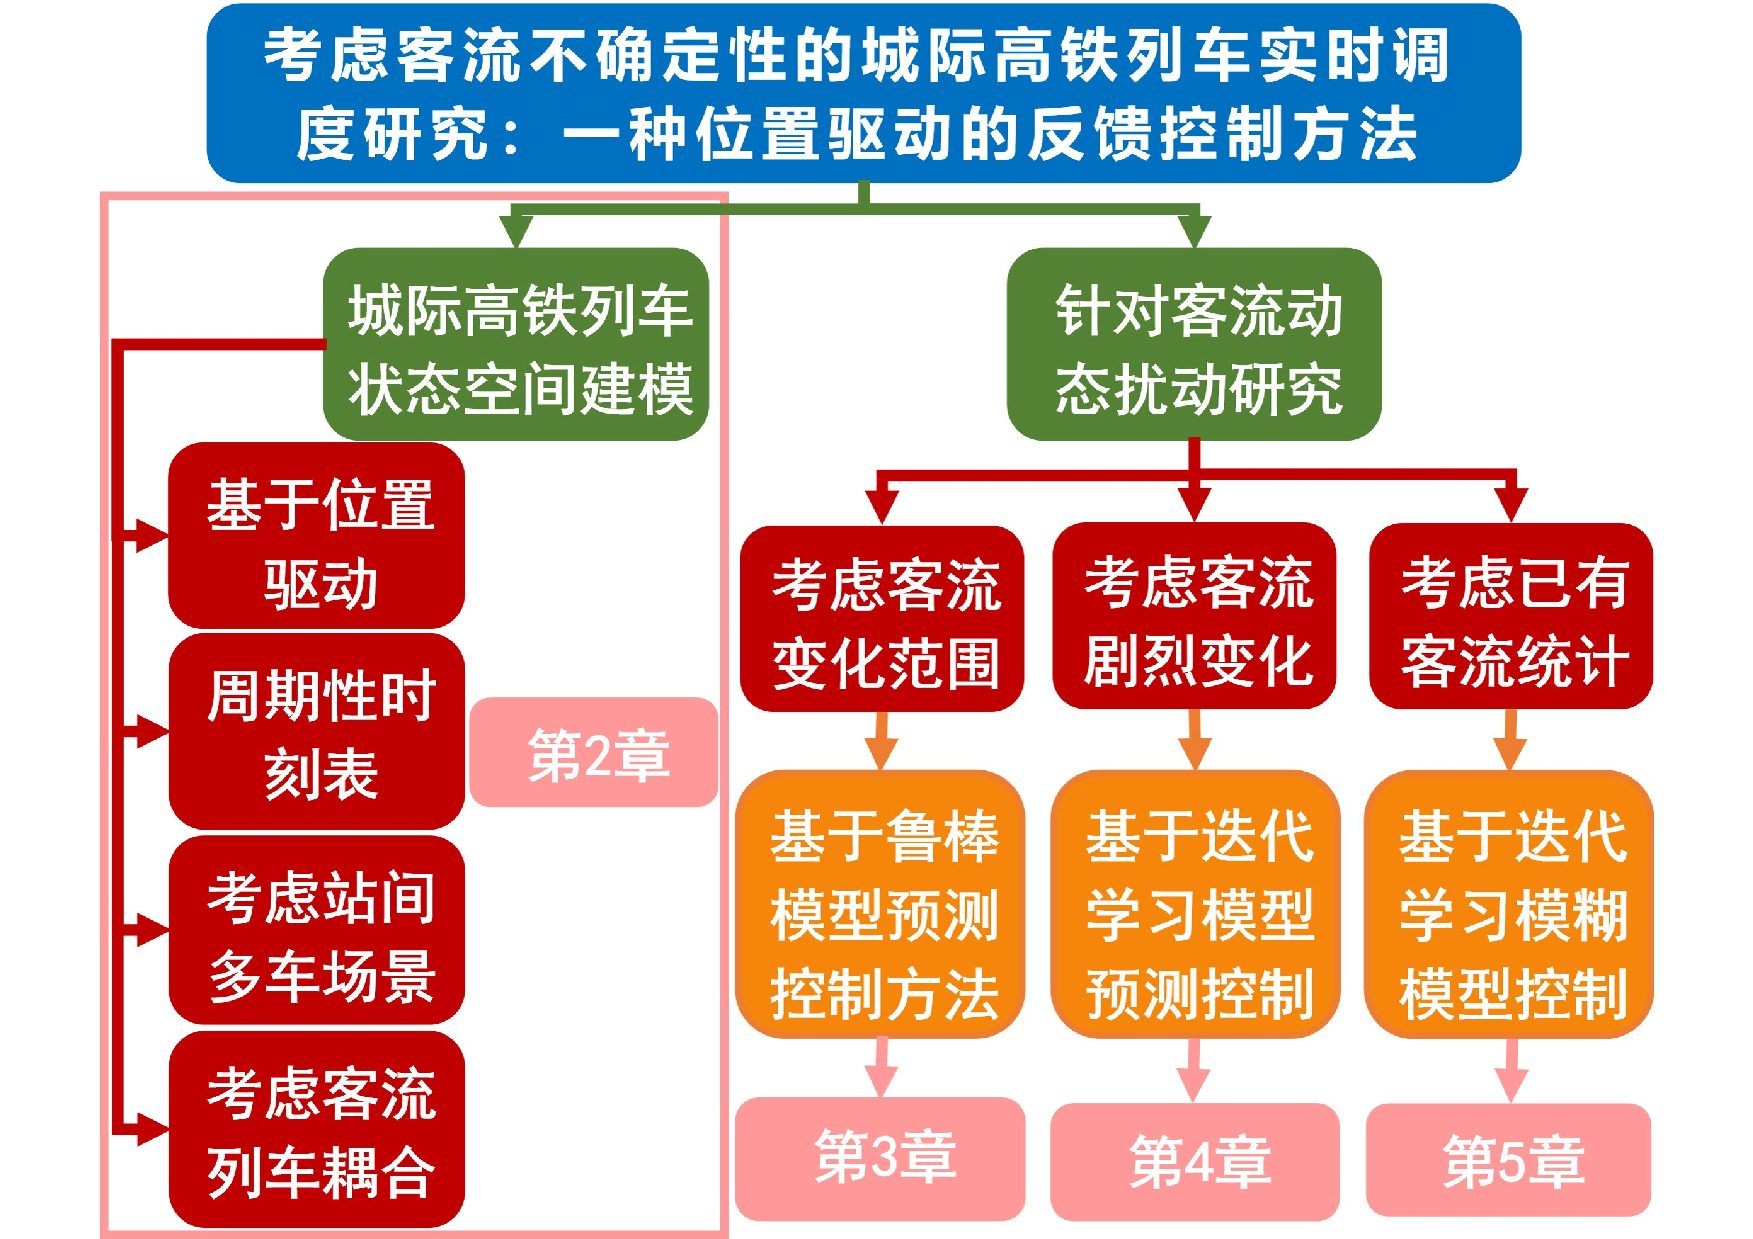
\includegraphics[width=\textwidth,height=0.7\textwidth]{Img/ch1/structure.pdf}
    \bicaption{本文研究内容组织结构图}{The organizational structure diagram of the research content in this paper}
    \label{fig1-n}
\end{figure}
